The processor presented as a solution for assignment 1 in this report is a simple 32-bit MIPS-inspired multi-cycle processor described in VHDL.
It was attempted programmed onto a Xilinx Spartan-6 LX25 FPGA.

\section{Solution Architecture}

The processor architecture is a MIPS-inspired pipelined architecture with five stages.
The five stages are called Instruction Fetch, Instruction Decode, Execution, Memory and Write Back.
Each stage is separated by pipeline registers that hold the relevant data for the different stages between clock cycles.
Since the the CPU is pipelined, it can achieve much higher performance than the simple multi-cycle processor architecture designed in the previous assignment\cite{assignment-1}.
For ideal execution, every component of the processor is in use in every cycle, giving a high utilization of resources.
Paradoxically, even though pipelined processor designs can be much more performant than simple multi-cycle processor designs, they are not necessarily more complex.
This is because there is no longer need for a massive state machine in the control unit in the pipeline processor, as there would be in a multi-cycle processor control unit.

Not everything is better with a pipelined design, however.
With a pipelined design, the processor is vulnerable to data hazards and control hazards.
A hazard, in processor design terminology, is a situation where a planned execution in a processor cannot be performed because it is dependant on the outcome of a previous execution which has not yet completed.
This is made possible because of the introduction of instruction-level parallelism.
The solution processor presented in this report resolves hazards by using a combination of data forwarding and stalling.
One type of hazard, the use-after-load\cn hazard, where an instruction relies on the data from a memory load in the instruction immediately preceding it, is not handled by the processor.
Trying to execute an instruction which uses the result from a load immediately after the load instruction results in undefined behaviour.
Instead of handling this in hardware, the bundled solution assembler solves this issue by instruction reordering, or simply inserting nops where needed.
This is done to remove complexity from the processor core, which in turn increases processor performance, which is aligned with the performance goal from section \vref{subsection:performance}.

The processor architecture is modeled after the Harvard Architecture design, which means that it has separate instruction and data memory.
This, in addition to being a security boon, makes for a more performant design, as the instruction memory and data can be accessed independently.
This is aligned with the performance design goal from \vref{subsection:performance}.

Having separate memories for data and instructions also removes the need for a central memory access arbitrage unit, which increases the simplicity of the design in accordance to the design goal in section\vref{subsection:simplicity}.

The processor architecture can bee seen illustrated in figure \vref{figure:architecture}.
The tall orange bars are the pipeline registers.
The blue lines are control signals.

\begin{figure}[H]
    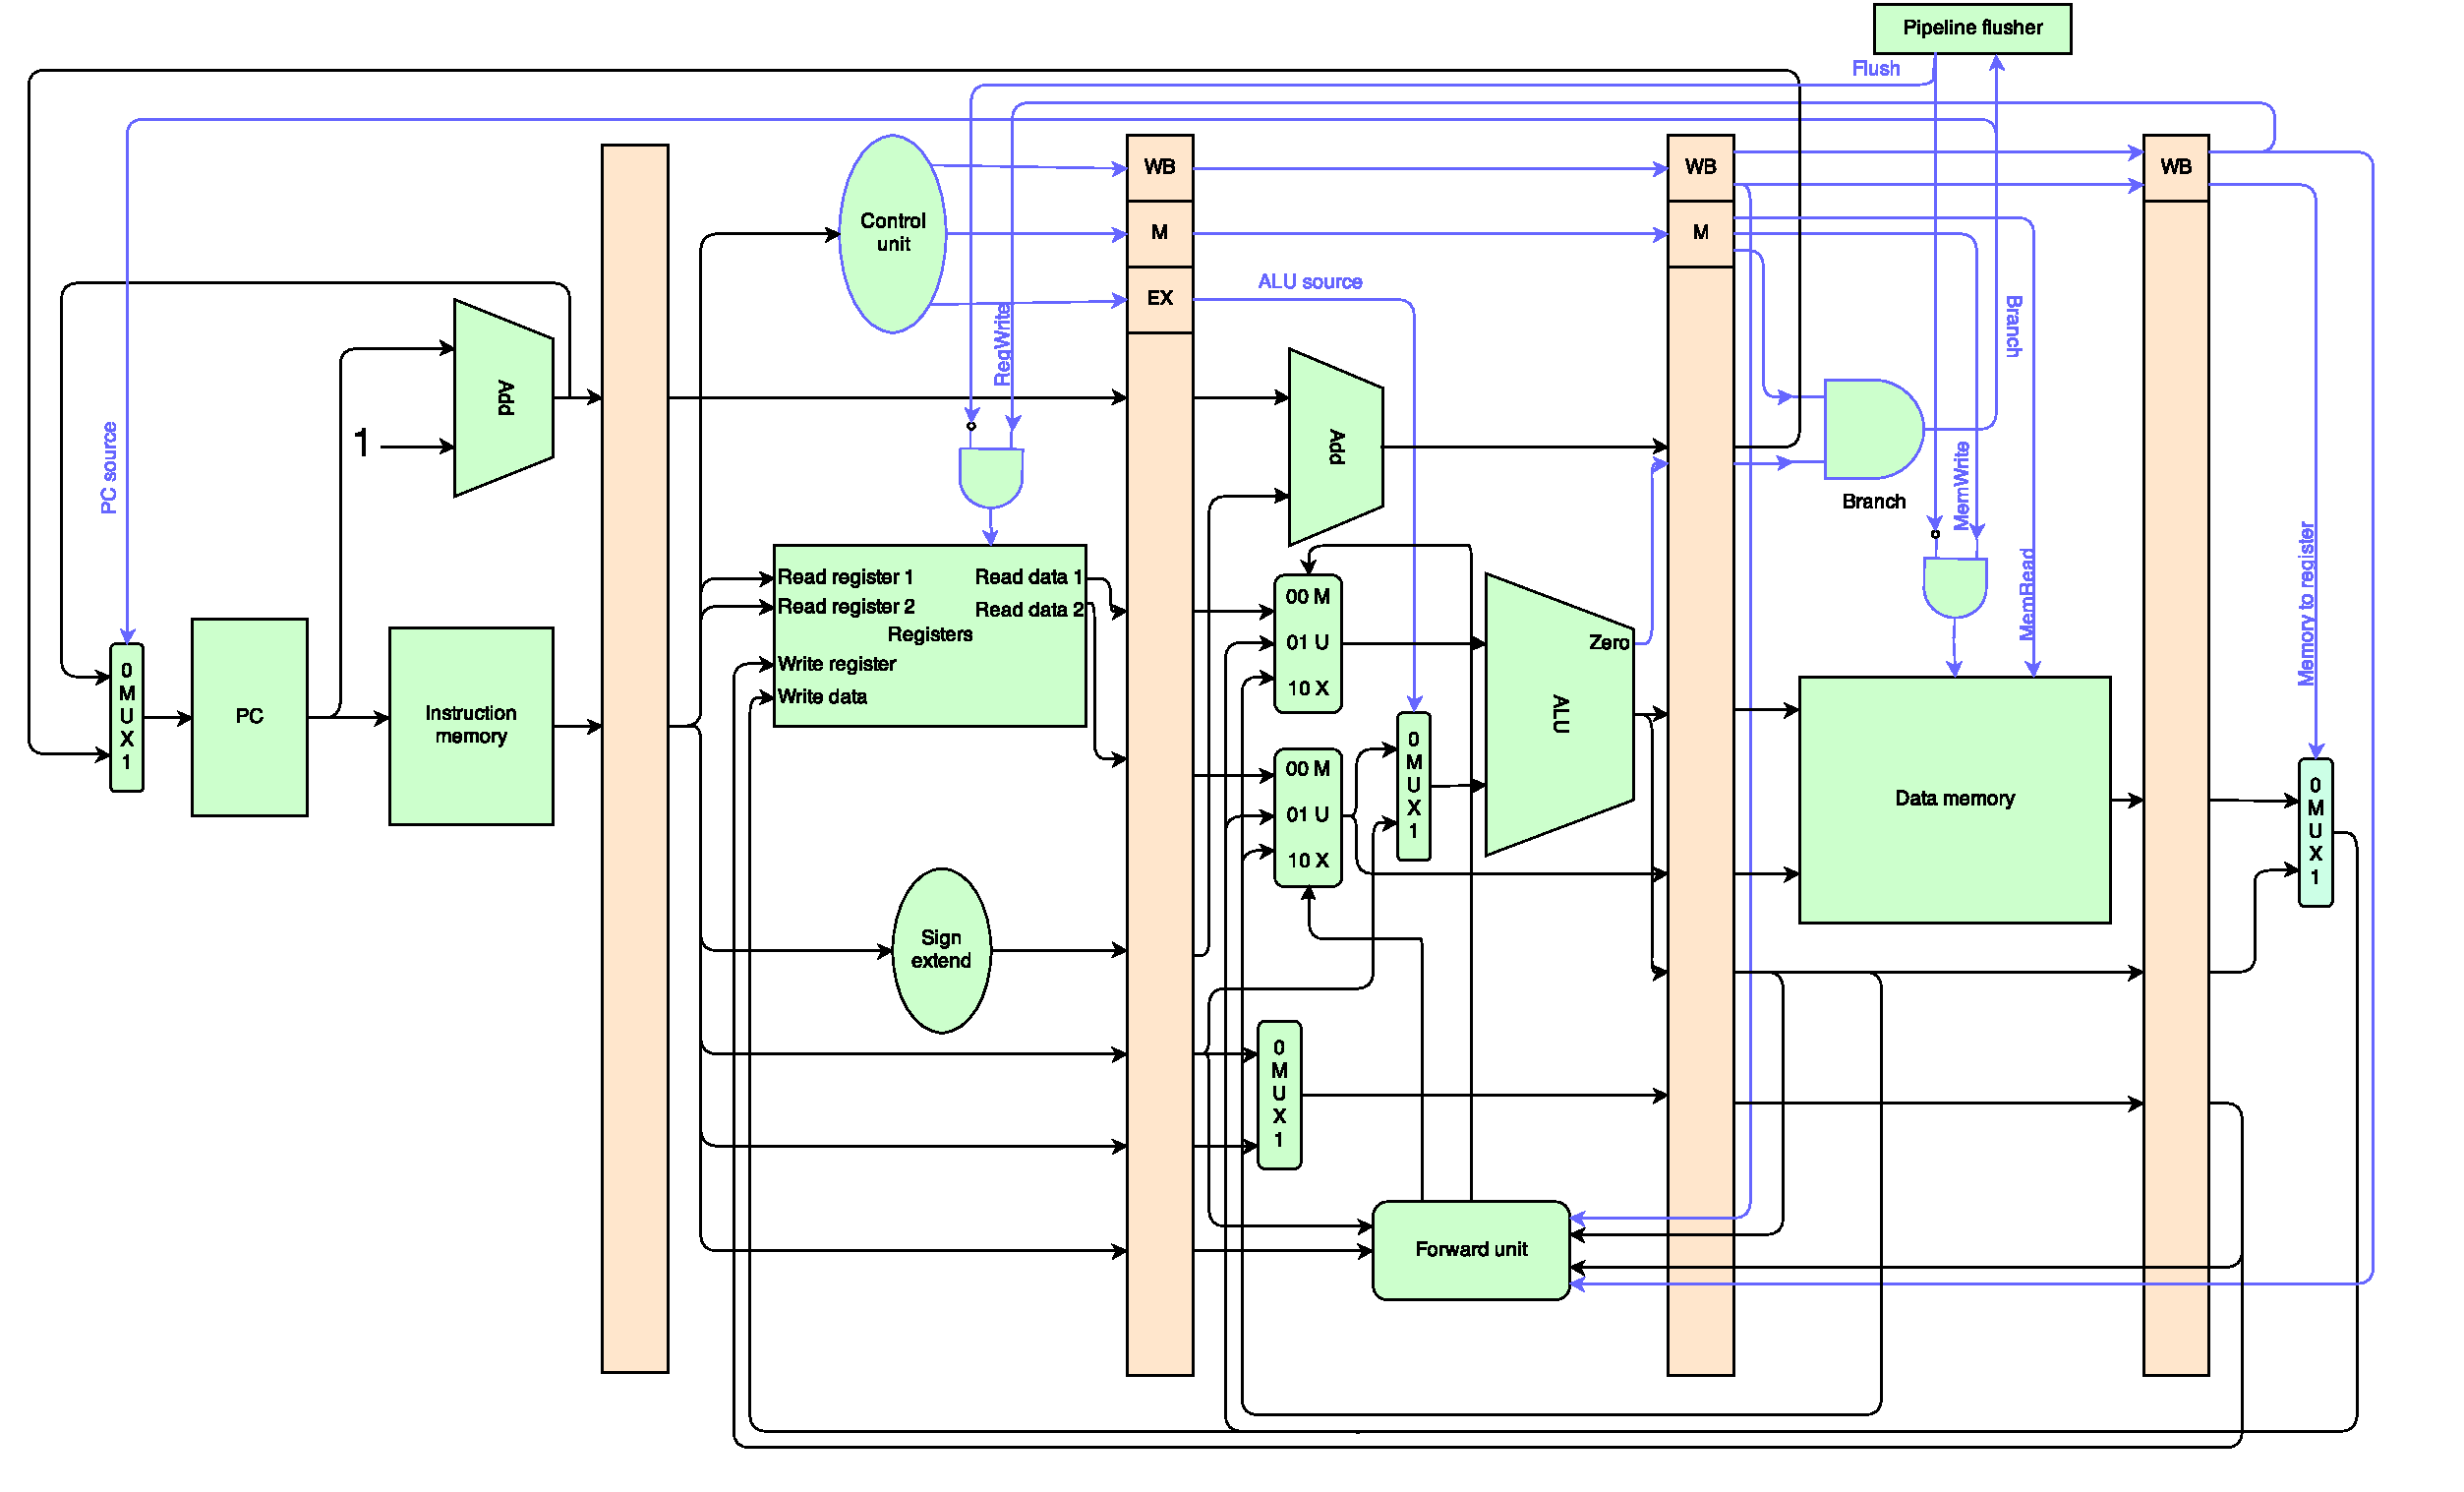
\includegraphics[width=\textwidth]{illustrations/processor.pdf}
    \caption{The processor architecture}
    \label{figure:architecture}
\end{figure}


The rest of this section describes the different architectural sub-components in detail.

\subsection{Instruction Fetch Stage}
    The instruction fetch stage is the first stage in the processor pipeline.
It is responsible for fetching the correct instruction from the instruction memory, and feeding it to the next stage in the pipeline.

\subsubsection{Program Counter}
In order to know where in the program the processor is currently executing, a program counter is needed.
The program counter is a simple register which holds the instruction address of the address currently being fetched and sent on to the next stage in the pipeline.
The instruction fetch stage updates the program counter each cycle, either by increasing it by one so as to fetch the next instruction, or by to a different number requested by a different part of the processor, in the case of a jump.



\subsection{Instruction Decode Stage}
    \todo{picture of decode stage}

The instruction decode stage receives an instruction from the instruction fetch stage and understands it.
Using this understanding, it orchestrates and coordinates the execution of the instruction.
This means that it is responsible for preparing the necessary data for the ALU, and setting the appropriate control signals for the rest of the processor for each instruction.
The register file of the processor resides in the instruction decode stage, and register data that are needed in computation in the execution stage are fetched and prepared in the instruction decode stage.
The control unit also resides in this stage.

\newpage
\subsubsection{Register File}
    The register file is a large block of 32 registers that make up the general purpose registers of the processor that are accessible to users.
The register file implementation is the same as in the prevous assignment\cite{assignment-1}, and is also part of the supplied support files for this assignment.


\newpage
\subsubsection{Control Unit}
    The control unit is the component that is responsible for enabling and disabling the correct parts of the processor at the correct times, so that an instruction is executed correctly.

\subsubsection{In Signals}

\begin{description}
\item{\textbf{Instruction Op-code}} \\
    The op-code of the currently executing instruction in the instruction decode stage.

\item{\textbf{Instruction Function}} \\
    The ALU function of the currently executing instruction in the instruction decode stage. 
\end{description}

\subsubsection{Out Signals}

\begin{description}
\item{\textbf{Execute Control Signals}} \\
    The control signals that should be used in the execute stage for the instruction being decoded by the control unit.
    The execute control signals bus contains the \textbf{ALU Source}, \textbf{ALU Function} and \textbf{Register Destination} control signals.

\item{\textbf{Memory Control Signals}} \\
    The control signals that should be used in the memory stage for the instruction being decoded by the control unit.
    The memory control signals bus contains the \textbf{Branch} and \textbf{Memory Write} control signals.

\item{\textbf{Write-Back Control Signals}} \\
    The control signals that should be used in the write-back stage for the instruction being decoded by the control unit.
The write-back control signals bus contains the \textbf{Memory to Register} and \textbf{Register Write} control signals.

\item{\textbf{Jump}} \\
    Whether or not the instruction being decoded is a jumping instruction (i.e. \texttt{JMP}).
\end{description}




\subsection{Execution Stage}
    \todo{describe this stage}
\todo{image of this stage}

\subsubsection{ALU}
    \todo{The ALU description}

\subsubsection{In Signals}

\begin{description}
\item{\textbf{Signal}} \\
Description of it.

\end{description}

\subsubsection{Out Signals}

\begin{description}
\item{\textbf{Signal}} \\
Description of it.
\end{description}


\subsubsection{Forwarding Unit}
    The forwarding unit is responsible for forwarding newly computed data from later stages in the pipeline to earlier stages, where new instructions might need the data before they are commited to registers at the end of the pipeline.
The forwarding unit is essential to achieving a high performance pipelined design, as without it computations would either be wrong or slow.

The forwarding unit looks at which data is needed in the execution stage, and if the needed data has been updated down the pipeline but not in the register file, forwards the data to the ALU instead of the old data fetched from the register file by the instruction decode stage.
To be able to do this, the forwarding unit needs data from many different stages at once.

\subsubsection{In Signals}

\begin{description}
\item{\textbf{rs\_address\_from\_id\_ex}} \\
    The source register address of the Rs operand from the ID/EX pipeline registers.

\item{\textbf{rt\_address\_from\_id\_ex}} \\
    The source register address of the Rs operand from the ID/EX pipeline registers.

\item{\textbf{register\_destination\_from\_ex\_mem}} \\
    The destination register address from the EX/MEM pipeline registers.

\item{\textbf{register\_destination\_from\_mem\_wb}} \\
    The destination register address from the MEM/WB pipeline registers.

\item{\textbf{register\_write\_from\_ex\_mem}} \\
    The register write control signal from the EX/MEM pipeline registers.

\item{\textbf{register\_write\_from\_mem\_wb}} \\
    The register write control signal from the MEM/WB pipeline registers.
\end{description}

\subsubsection{Out Signals}

\begin{description}
\item{\textbf{forward\_rs\_out}} \\
    The forwarded value of the Rs register.

\item{\textbf{forward\_rt\_out}} \\
    The forwarded value of the Rt register.

\end{description}


\subsubsection{Hazard Detector}
    \todo{The Hazard Detector description}

\subsubsection{In Signals}

\begin{description}
\item{\textbf{register\_address\_in}} \\
Description of it.
\item{\textbf{register\_write\_execute\_in}} \\
Description of it.
\item{\textbf{register\_write\_memory\_in}} \\
Description of it.
\item{\textbf{register\_destination\_execute\_in}} \\
Description of it.
\item{\textbf{register\_destination\_memory\_in}} \\
Description of it.
\end{description}

\subsubsection{Out Signals}

\begin{description}
\item{\textbf{hazard\_out}} \\
Description of it.
\end{description}



\subsection{Memory Stage}
    \subsubsection{Data Memory}


\subsection{Write-Back Stage}
    The Write Back stage is responsible for routing the correct data to the register file, when data should be written to the register file.


\subsection{Additional Components}
    \subsubsection{Pipeline Registers}

Between each stage of the pipeline there are series of registers that hold the necessary values between clock ticks.
The pipeline registers are clocked synchronously, which means that the pipeline design is a buffered synchronous design.
The pipeline registers are implemented as flip-flops.


\subsubsection{Flip Flop}

A flip-flop is a simple circuit that has two stable states.
The implication is that they can be used to store values over time.

In the solution processor, size-generic flip-flops VHDL are used.
Because type generics were first introduced in the VHDL 2008 standard\cite{vhdl2008}, and the Xilinx tool chain doesn't support it yet, flip-flops are implemented on a per-type basis.
Subsequently, the \texttt{flip\_flop.vhd} VHDL source code file is a lot bigger and hairier than it could be.

\subsubsection{Multiplexers}

A multiplexer is a component which selects between multiple input signals based on a separate control signal.
Since multiplexers are use quite commonly, and VHDL has no build in construct for it, some multiplexer components are introduced in the solution.

\subsubsubsection{Multiplexer 2}

The Multiplexer 2 selects one of two possible input values based on the value of a 1-bit selection signal.

\subsubsubsection{Multiplexer 3}

The Multiplexer 3 selects one of three possible input values based on the value of a 2-bit selection signal.
Since a 2-bit selection signal may have 4 possible states, and the Multiplexer 3 only has three inputs, one of the selection signal states ("\texttt{11}") holds undefined behaviour.

\subsubsection{Pipeline flusher}

The pipeline flusher is reponsible for flushing the pipeline if a branch prediction goes wrong.
In such a case, the pipeline will be filled with instructions that shouldn't be executed.
The pipeline flusher disables these instructions by removing their ability to write to registers and memory.




\subsection{ALU}

Something about the alu. We could mention that we rewrote it because of reasons?

\subsection{Control Unit}

The control unit is a finite state machine that controls the processor.
Its job is to maintain the control state across cycles, and distribute the correct control signals to the other components in the processor at the right time.
The finite state machine has three states: fetch, execute and stall.
It advances to the next state on every cycle, with transitions as illustrated in figure \ref{figure:control-unit-state-machine}.

\begin{figure}[h]
    \begin{center}
        \begin{tikzpicture}[->,>=stealth',shorten >=1pt,auto,node distance=2.8cm, semithick]
            \tikzstyle{every state}=[fill=none,draw=black,text=black]
            \node[initial,state] (fetch)                    {$fetch$};
            \node[state]         (execute) [right of=fetch] {$execute$};
            \node[state]         (stall) [right of=execute] {$stall$};
            \path (fetch) edge node {} (execute)
                (execute) edge [bend left] node {non-mem} (fetch)
                (execute) edge node {mem} (stall)
                (stall) edge [bend right] node {} (fetch);
        \end{tikzpicture}
            \caption{
                Control unit state machine.
                \texttt{mem} transitions are taken when the currently executed instruction accesses memory.
            }
            \label{figure:control-unit-state-machine}
    \end{center}
\end{figure}

TODO: explain the signals that come out of the control unit

Here is a list for now populated by the signal names and Odd's educated guesses and brief explanations of the obvious.

\subsubsection{ALU Source}
The control signal for the ALU Source MUX. If 1 then the MUX selects the output from Sign Extend, if 0 it selects the signal from Read Data 2 in the Registers block.

\subsubsection{Register Write}
Does this turn on if we are writing to a register?

\subsubsection{Register Destination}
If 1 then the the Register Destination MUX outputs bits 15-11 of the instruction. If 0 then it outputs bits 20-16 of the instruction. Either way it feeds this to the Write Register port on the Registers block.

\subsubsection{Memory to Register}
Is this like, fetch? Are we putting memory in the registers?

\subsubsection{Memory Write}
I guess this is set if the instruction writes to memory?

\subsubsection{Jump}
The Jump signal indicates whether or not the current instruction is a jump instruction. If it is, the Jump signal is set to $1$ which causes the Jump MUX to output the Jump Address signal from Concat.

\subsection{Branch Controller}

The branch controller is the logic unit that decide whether or not the program should branch.
It is seperated from the main controller unit, as it works independently from the state machine (see Figure \ref{figure:control-unit-state-machine} and does not need to follow the clock.
The branch controller reads the opcode field from the instruction, and if it is a branch instruction it will run the logic that is requiered for that instruction.

To handle the simplest operations that compare two registers to each other, the branch controller can simply look at the flags from the ALU to decide if the branch mux should be enabled.
Instructions that compare a register to zero require a bit more work from the branch controller.
The branch controller can send out a zero value that overrides the ALUs source for the y operand, and is compared to the x operand from the register specified in the instruction.

To allow for other compare operations than $x \geq 0$ and $x < 0$, the zero vaule will not always be zero. 
Because the solution processor can only handle integers, $x \geq 1$ can be said to be equivalent with $x > 0$.
This trick means that there is no need to support more than zero and negative (TODO: ZERO AND NEGATIVE WHAT?), and can save quite a bit of complexity in our design without losing performance.
Therefore the zero value from the branch controller varies from -1 to 1. (TODO: WHAT?)

The control unit will assist the branch controller by instructing the ALU to do a subtraction on its inputs, $x - y$, and discard the result.
This will set the zero flag of the ALU if the $x = y$, and the negative flag of the ALU if the $x < y$.
These flags are used by the branch controller to determine whether it should branch or not.

\subsection{Program Counter Cycle}

The program counter cycle is the loop the program counter forms together with the branch and jump circuitry.
The program counter is a D-latch register (TODO: is it?) that holds the address of the next instruction to be fetched.
When no branching or jumping is involved (the ``sunny day scenario''), the program counter cycle increments the program counter by one every cycle the control unit tells it to.
This means that the control unit has the opportunity to advance the running program.
The control unit advances the program counter when it is in the execute state, so that a new program counter value is ready for when the control unit enters the fetch state.

When the control unit gives the signal, the program counter may perform a branch or a jump by manipulating the program counter cycle to change the value sent back to the program counter.

TODO: diagram of the program counter cycle.

\subsection{Multiplexer}

The multiplexer... do we even need to talk about it?

\section{Instruction Set}

The solution processor implements a modified subset of the MIPS instruction set.
A quick reference of the MIPS instruction set can be found in Figure 3.4 of the compendium \cite{compendium}.
The instructions, as in regular MIPS, can be on one of three general formats, R, I and J.

The solution processor implements the instructions in table \ref{table:implemented-instructions}.
The processor supports quite a few more instructions than the minimum requirements.
This is done because (TODO: convincing argument).

\begin{table}
    \begin{center}
        \begin{tabular}{r|l}
            \texttt{ADD} & Add \\
            \texttt{ADDI} & Add immediate \\
            \texttt{ADDIU} & Add immediate unsigned \\
            \texttt{ADDU} & Add unsigned \\
            \texttt{AND} & And \\
            \texttt{ANDI} & And immediate \\
            \texttt{BEQ} & Branch if equal \\
            \texttt{BNE} & Branch not equal \\
            \texttt{J} & Jump \\
            \texttt{LUI} & Load upper immediate \\
            \texttt{LW} & Load word \\
            \texttt{MULT} & Multiply \\
            \texttt{MULTU} & Multiply unsigned \\
            \texttt{NOR} & Nor \\
            \texttt{OR} & Or \\
            \texttt{ORI} & Or immediate \\
            \texttt{PASSTHROUGH} & Passthrough (i.e. send the first input through unmodified) \\
            \texttt{SLL} & Shift left logical \\
            \texttt{SLLV} & Shift left logical variable \\
            \texttt{SLT} & Set less than \\
            \texttt{SLTI} & Set less than immediate \\
            \texttt{SLTIU} & Set less than immediate unsigned \\
            \texttt{SLTU} & Set less than unsigned \\
            \texttt{SRA} & Shift right arithmetic \\
            \texttt{SRAV} & Shift right arithmetic variable \\
            \texttt{SRL} & Shift right logical \\
            \texttt{SRLV} & Shift right logical variable \\
            \texttt{SUB} & Subtract \\
            \texttt{SUBU} & Subtract unsigned \\
            \texttt{SW} & Store word \\
            \texttt{XOR} & Xor \\
            \texttt{XORI} & Xor immediate \\
        \end{tabular}
        \smallskip
        \hrule
        \smallskip
        \caption{Implemented instructions}
        \label{table:implemented-instructions}
    \end{center}
\end{table}

\section{Test utilities}

TODO: move the solution component description of the test utilities from results-and-tests here

\section{Deliverables}

This is where we list all the deliverables we're sending in.
